\section{$\hat{C}\hat{P}$V in Kaon System} 

\subsection{Neutral Kaon Mixing}

As mentioned $\hat{C}\hat{P}$V was first observed in the neutral kaon system. Direct and indirect $\hat{C}\hat{P}$V have been observed but it is found that the process is entirely dominated by the indirect method [Zeng, need better reference]. Essential to these mechanisms is the mixin
g between the neutral Kaon and its anti-particle, corresponding to the states $\ket{K^{0}}$ and $\ket{\bar{K}^{0}}$. These have quark compositions of $d \bar{s}$ and $s \bar{d}$, respectively. 

In interactions involving the strong or EM force, the quantum number strangeness, which tells us the number of strange quarks in a particle, must be conserved. For the weak force it is found that, like parity, this symmetry is not conserved. Due to this many processes forbidden for the strong and EM interactions are allowed through the weak force. This violation is what makes mixing possible. Mixing is the decay of a particle into its anti-particle and can only take place when a particle is its own anti-particle, or if the particles differ by a quantum number which is not conserved by some interaction. This is the case in neutral Kaon mixing, also know as Kaon oscillations. The neutral Kaon and its anti-particle have opposite strangeness but can decay into each other through the strangeness violating weak force. See Fig.(add in feynman digram of M+S pg 289) 

Analogous to the mixing of mass eigenstate quarks to different quark flavours, it is found that the neutral Kaon flavour eigenstates do not correspond to eigenstates of the $\hat{C}\hat{P}$ operator. To show this we first operate on the Kaon states with the $\hat{C}$ operator. We first assume that there is no $\hat{C}\hat{P}$V, then neglecting phase throughout we obtain:

\begin{align*}
\hat{C} \ket{K^{0}(d \bar{s})} = (1)(-1) \ket{\bar{K}^{0}(s \bar{d})} = - \ket{\bar{K}^{0}(s \bar{d})}  \\
\hat{C} \ket{\bar{K}^{0}(s \bar{d})} = (1)(-1) \ket{K^{0}(d \bar{s})} = - \ket{K^{0}(d \bar{s})}  
\end{align*}

\noindent Where we have used the convention that $\hat{C} (q) = 1$ and $\hat{C} (\bar{q}) = -1$. Also, the action of the $\hat{P}$ is given by:
    
\begin{align*}
\hat{P} \ket{K^{0}(d \bar{s})} = \hat{P}(d) \hat{P}(\bar{s})(-1)^{l} \ket{K^{0}(d \bar{s})} = (1)(-1)(-1)^0 \ket{K^{0}(d \bar{s})} = - \ket{K^{0}(d \bar{s})} \\
\hat{P} \ket{\bar{K}^{0}(s \bar{d})} = \hat{P}(s) \hat{P}(\bar{d})(-1)^{l} \ket{\bar{K}^{0}(s \bar{d})} = (1)(-1)(-1)^0 \ket{\bar{K}^{0}(s \bar{d})} = - \ket{\bar{K}^{0}(s \bar{d})} 
\end{align*}

\smallskip

\noindent Where we have used the convention $\hat{P} (fermion) = 1$ and $\hat{P} (anti-fermion) = -1$ as well as $l=0$ because the Kaon is the lowest energy combination of these quarks and itself has a $J^{P}$ pf $0^{-}$. Now we are in a position to determine the eigenstates of $\hat{C}\hat{P}$:

\begin{align*}
\hat{C}\hat{P} \ket{K^{0}} = \ket{\bar{K}^{0}} \\
\hat{C}\hat{P} \ket{\bar{K}^{0}} = \ket{K^{0}} 
\end{align*}

\noindent So we can see that any eigenfunction of the $\hat{C}\hat{P}$ operator will be a linear combination of the two Kaon states:

\begin{align}\label{FirstKaonLinComb}
\ket{K^{0}_{1}} = \frac{1}{\sqrt{2}} (\ket{K^{0}} + \ket{\bar{K}^{0}}) \\
\ket{K^{0}_{2}} = \frac{1}{\sqrt{2}} (\ket{K^{0}} - \ket{\bar{K}^{0}})
\end{align} 

\noindent Where 1 and 2 are the usual labels given to these states. Now we investigate the action of $\hat{C}\hat{P}$ on these linear combinations

\smallskip

\begin{align*}
\hat{C}\hat{P} \ket{K^{0}_{1}} & = \frac{1}{2} (\hat{C}\hat{P} \ket{K^{0}} + \hat{C}\hat{P} \ket{\bar{K}^{0}}) = \frac{1}{2} (\ket{\bar{K}^{0}} + \ket{K^{0}}) = \ket{K^{0}_{1}} \\
\hat{C}\hat{P} \ket{K^{0}_{2}} & = \frac{1}{2} (\hat{C}\hat{P} \ket{K^{0}} - \hat{C}\hat{P} \ket{\bar{K}^{0}}) =   \frac{1}{2} (\ket{\bar{K}^{0}} - \ket{K^{0}}) = - \ket{K^{0}_{2}} \\
\end{align*} 

In experiment, two Kaon states are observed, a short lived state denoted by $\ket{K^{0}_{S}}$ and a relatively long lived state, $\ket{K^{0}_{L}}$. The lifetimes of these particles are $8.954 \pm 0.004 \e{−11}~$s and $5.116 \pm 0.021 \e{−8}~$s \cite{PDGKaons}. We make the natural assumption that these are the $\hat{C}\hat{P}$ eigenstates just derived. We make the identifications $\ket{K^{0}_{S}} = \ket{K^{0}_{1}}$ and $\ket{K^{0}_{L}} = \ket{K^{0}_{2}}$ and see what this predicts. If $\hat{C}\hat{P}$ is conserved then all the decays of the $\ket{K^{0}_{S}}$ ($CP = 1$) state must be to final products with $CP = 1$, and similarly, the decays of $\ket{K^{0}_{L}}$ ($CP = -1$) must be to final products with $CP = -1$. The observed decays for these states are as follows \cite[pg. 292]{Martin+Shaw}:

\begin{eqnarray*}    
K^{0}_S \rightarrow \pi^0 \pi^0 (B = 0.31),  &   &   K^{0}_{S} \rightarrow \pi^{+} \pi^{-} (B = 0.69)\\ [6pt]
K^{0}_L \rightarrow \pi^0 \pi^0 \pi^0 (B = 0.20),   &   &   K^{0}_{L} \rightarrow \pi^{+}  \pi^{-} \pi^0 (B =0.13)  
\end{eqnarray*}    

\noindent The reason for the difference in lifetimes of these two Kaon states is that the mass of the $K^{0}_L$ is not much bigger than the mass of three pions, thus it is relatively unlikey for it to undergo decay, compared to the $K^{0}_S$ which must only create energy to make two pions. We now determine the $CP$ of these final states. This is easy for the two pion final states. We find:

\begin{align}
{P} ({\pi^0 \pi^0})   = & (-1)(-1)(-1)^{l=0} = +1 & \Rightarrow P = 1  \\
{C} ({\pi^0 \pi^0})   = & 1                       & \Rightarrow C = 1  \\
{P} ({\pi^+ \pi^-})   = & (-1)(-1)(-1)^{l=0} = +1 & \Rightarrow P = 1  \\
\label{TwoPionFinalStateCalc}
{C} ({\pi^+ \pi^-})   = & (-1)^{l=0}             & \Rightarrow C = 1 
\end{align}

\noindent Thus $\hat{C}\hat{P} \ket{\pi \pi} = 1$. Now for the three pion final state we must take account of the second orbital angular momentum introduced by the  third pion. The general formula for such a system is $\hat{P} (ABC) = \hat{P} (A) \hat{P} (B) \hat{P}(C) (-1)^{\mathbf{L}_{AB}} (-1)^{\mathbf{L}_{(AB)C}}$ where $\mathbf{L}_{AB}$ is the orbital angular momentum of the first two pions and $\mathbf{L}_{(AB)C}$ is the orbital angular momentum of the third pion with respect to the mutual centre of mass of the first two pions. The $J^{P}$ of the Kaon is $0^{-}$, thus the overall orbital angular momentum must be zero: $\mathbf{L} = \mathbf{L}_{AB} + \mathbf{L}_{(AB)C} = 0$. As this is angular momentum addition and $\mathbf{L}$ can only take positive values, we conclude that ${L}_{AB} = {L}_{(AB)C}$ so ${L}_{AB} + {L}_{(AB)C} = 2L$, which is an even number: 

\begin{align*}
P(\pi^0 \pi^0 \pi^0)  = & (-1)(-1)(-1)(-1)^{2L = even} = -1 & \Rightarrow P = -1 \\
C(\pi^0 \pi^0 \pi^0)  = & (1)(1)(1) = 1                     & \Rightarrow C = +1 \\
CP(\pi^0 \pi^0 \pi^0) = & -1                                &
\end{align*}

\noindent For the $\ket{\pi^+ \pi^- \pi^0}$ final state the parity is also -1, but the charge conjugation picks up an extra factor of $(-1)^{l}$ as in Eqn.(\ref{TwoPionFinalStateCalc}). So if we take the centre of mass of pions A and B to be the centre of mass between the $\pi^{+}$ and $\pi^{-}$ we obtain:

\begin{align*}
C(\pi^+ \pi^- \pi^0)  = & C(\pi^{0})(-1)^{{L}_{AB}} = 1     & \Rightarrow C = +1 \\
CP(\pi^0 \pi^0 \pi^0) = & -1                                &
\end{align*}
 
\noindent Where ${L}_{AB} = 0$ is an experimentally determined quantity [Verify: ``Measurement of the $1H(\gamma,\pi^{0})$ cross section near threshold. II. Pion angular distributions'' - J. C. Bergstrom, R. Igarashi, and J. M. Vogt , Phys. Rev. C 55, 2016–2023 (1997)]. Thus as long as $K^{0}_{L}$ deacy to final states with three pions or other $CP = -1$ states and $K^{0}_{S}$ only decay to two pion final states or other $CP = 1$ states, then $CP$ is conserved.

This was thought to be the case until in 1964 when Christenson et al discovered the decay mode $K^{0}_{L}(CP = -1) \rightarrow \pi^+ \pi^- (CP = 1)$ with a branching ratio of $(2.3 \pm 0.3) \e{-3}$, thus discovering CP violation for the first time \cite{FirstCPV}. The experiment exploits the difference in lifetimes between $K^{0}_{S}$ and $K^{0}_{L}$. A 30GeV proton beam is incident on a metal target which creates a secondary beam of many different particles. The centre of mass energy for such an arrangement is $787~$MeV, which is more than enough energy to produce a neutral Kaon having about a $497~$MeV rest mass. The secondary beam is passed through a magnetic field to remove any charged particles and through a $4~$cm thick block of lead to remove photons. At this point the beam contains both $K^{0}_{S}$ and $K^{0}_{L}$. The detecting aparatus is placed $18~$m away from the metal target, so by the time the beam reaches it, all of the $K^{0}_{S}$ have decayed and only $K^{0}_{L}$ remain. The beam is further collimated and then undergoes collisions in a helium filled bag. Two arms containing a series of detectors are mounted symmetrically around the helium bag, so they both make the same angle with the horizontal. These arms consist of a spark chamber and magnet to determine the momentum and direction of an incident particle. Water Cherenkov and scintillation detectos act as a trigger by only recording events with two oppositely charged particles and a velocity of $0.75~$c to eliminate background, see Fig.(\ref{Christenson_apparatus}). The aim of the experiment is to measure the angular distribution of produced particles. The results of the experiment are shown in Fig.(\ref{Christenson_results}) where N is the number of counts and $\theta$ is the angle between the net momentum of the detected particles and the initial beam direction. These measurements were taken in various mass ranges, two are shown. If $K^{0}_{L} \rightarrow \pi^+ \pi^-$ is observed, the detected particles will have opposite signs, their invariant mass will match that of $K^{0}_{L}(497)$ and their net momentum will be in the same direction as the incident beam, hence the measured angle will be zero. We see from the results that a peak occurs at an angle of $0^{\circ}$ in the correct mass range. This is clear evidence of the $CP$ violating decay $K^{0}_{L} \rightarrow \pi^+ \pi^-$.   

\begin{figure}[h!]
\begin{center}
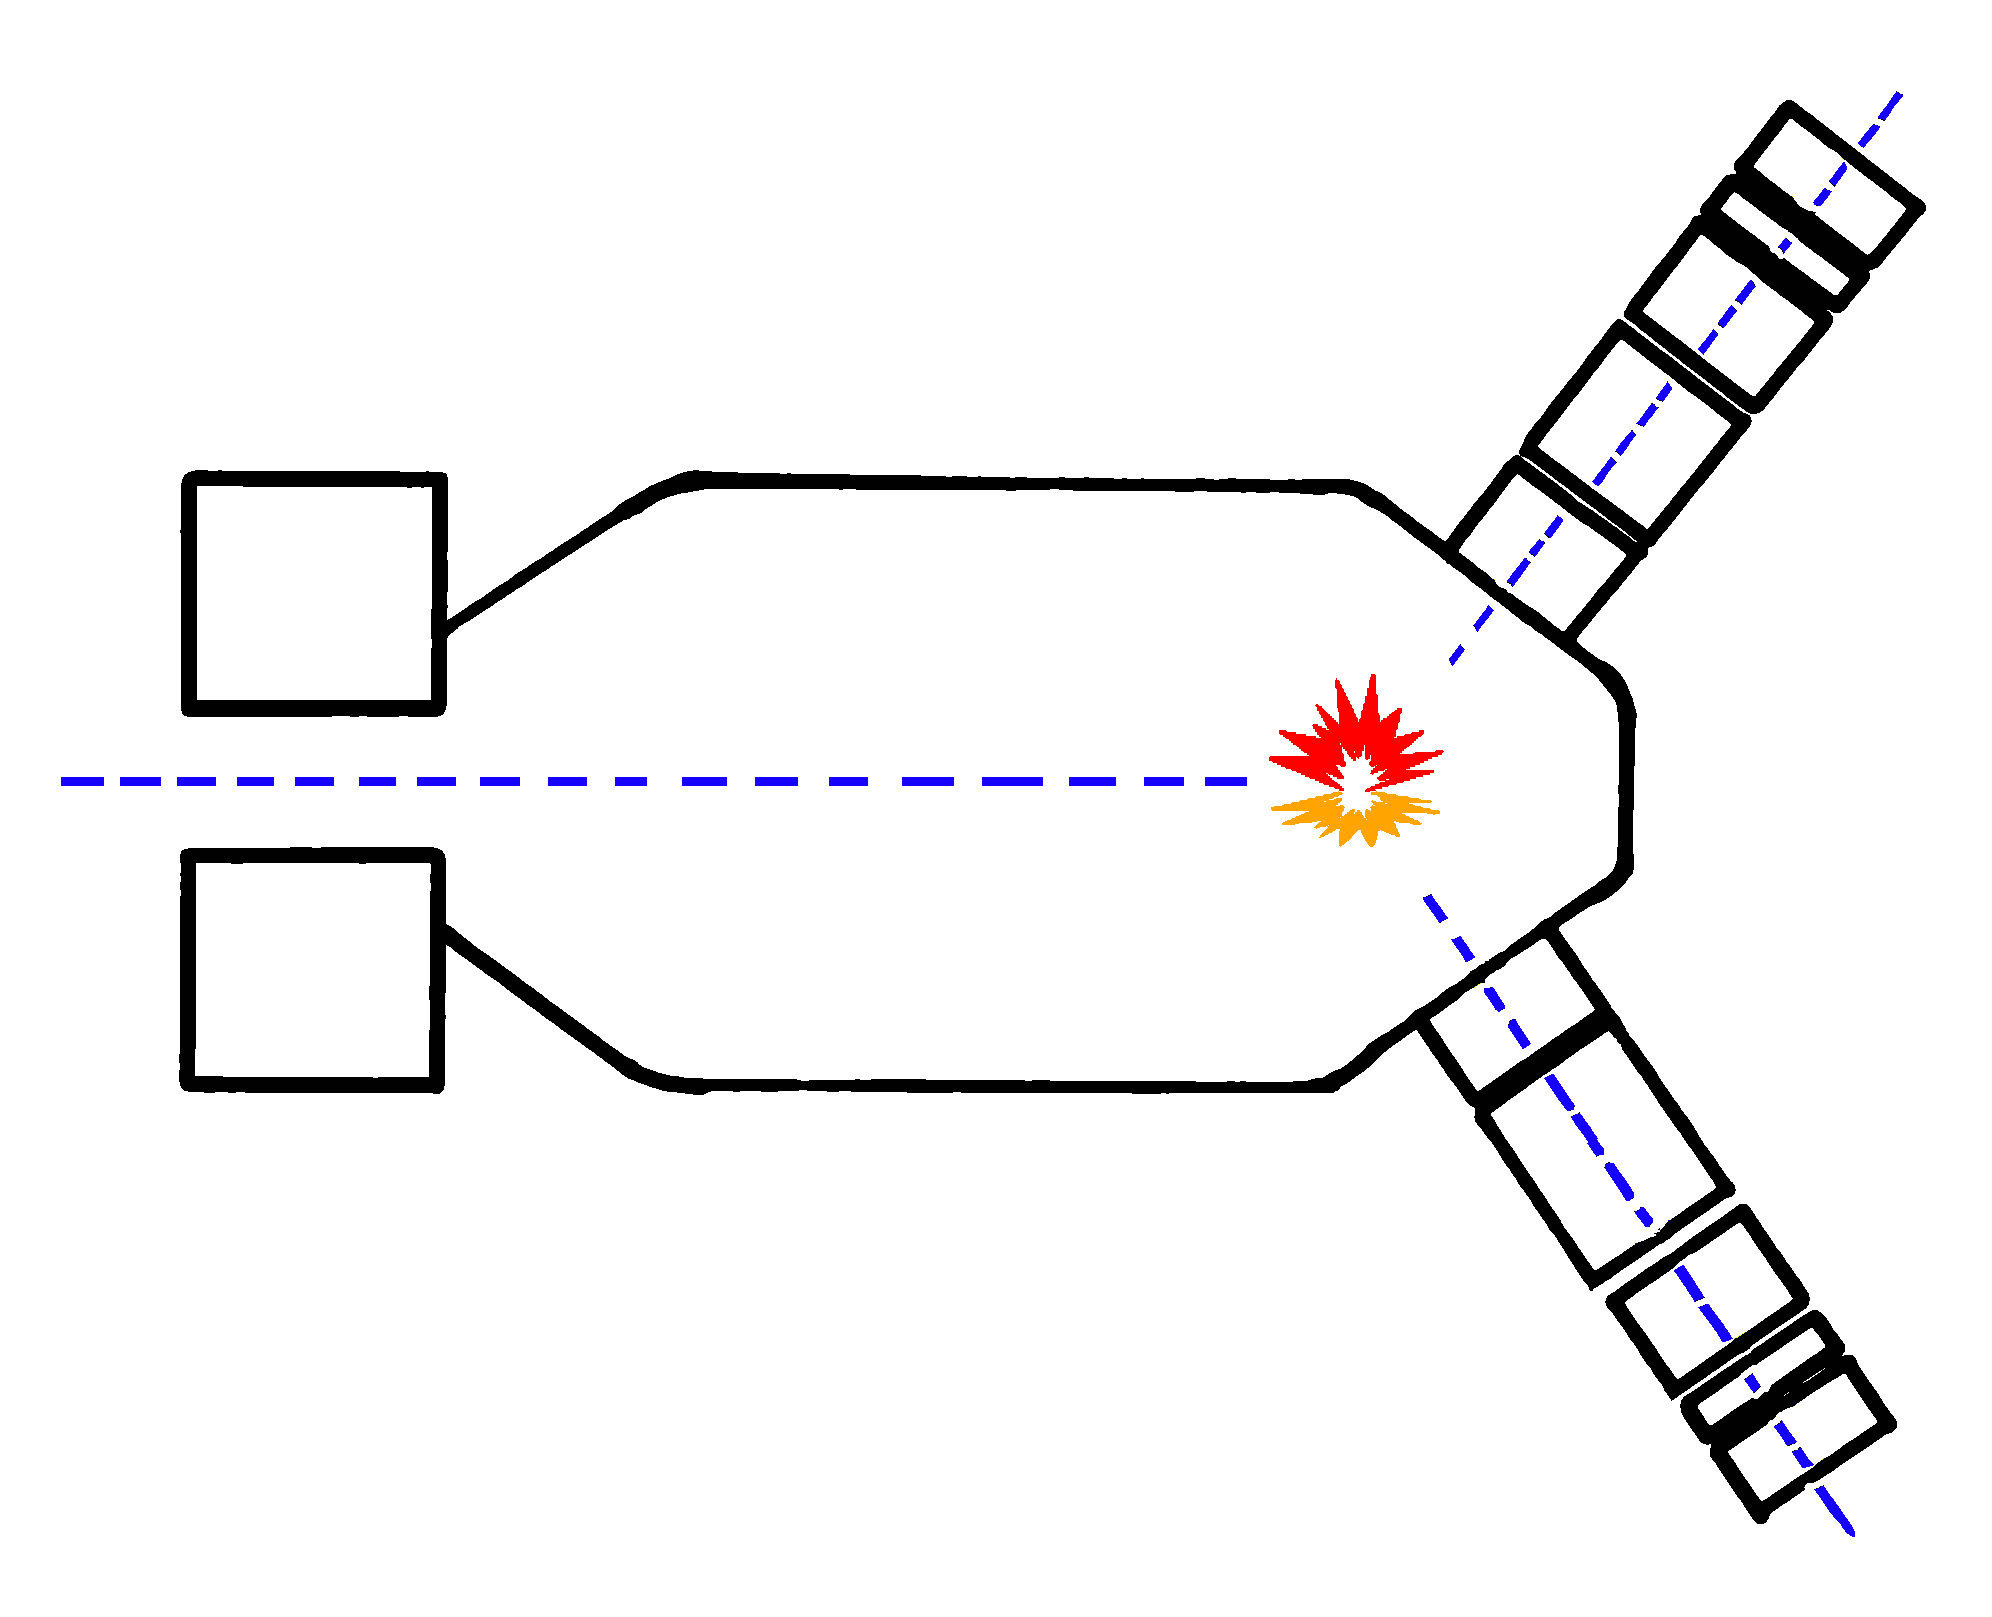
\includegraphics[scale=0.1]{figs/Christenson_apparatus.png}
\end{center}
\caption{\textit{Apparatus used in the Christenson et al experiment \cite{Christenson_apparatus_ref}}}
\label{Christenson_apparatus}
\end{figure}

\begin{figure}[h!]
\begin{center}
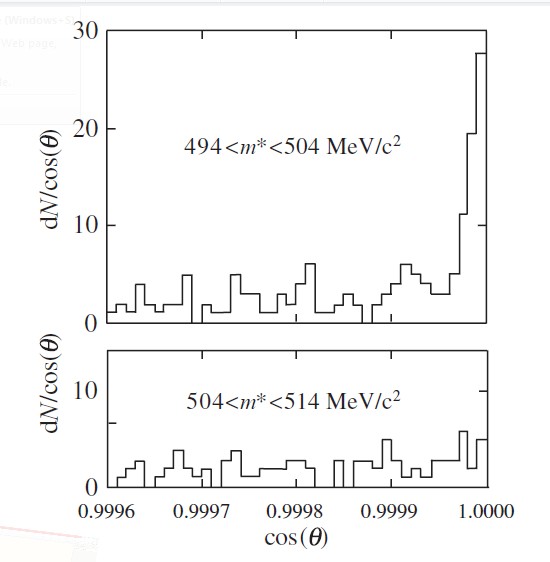
\includegraphics[scale=0.3]{figs/Christenson_results.png}
\end{center}
\caption{\textit{Results of the Christenson et al experiment \cite{FirstCPV}}}
\label{Christenson_results}
\end{figure}

The results of the Christensen et al experiment implies, that the weak eigenstates $\ket{K^{0}_{S}}$ and $\ket{K^{0}_{L}}$ are not aligned with the true $CP$ eigenstates $\ket{K^{0}_{1}}$ and $\ket{K^{0}_{2}}$. As in Eqn.(\ref{FirstKaonLinComb})  we write:

\begin{align}
\label{KaonLincomb11}
\ket{K^{0}_{S}} = a \ket{K^{0}_{1}} + b \ket{K^{0}_{2}} \\
\label{KaonLincomb12}
\ket{K^{0}_{L}} = a \ket{K^{0}_{1}} - b \ket{K^{0}_{2}}
\end{align}

\noindent Where $a$ and $b$ are complex numbers. We can determine the degree to which the states are not aligned using the CP violation decay amplitudes and corresponding CP conserving amplitudes \cite{Measurements_Direct_CPV_Kaons_KTev}: 

\begin{align*}
\eta_{+-} \vcentcolon= \frac{A(K^{0}_L \rightarrow \pi^+ \pi^-)}{A(K^{0}_S \rightarrow \pi^+ \pi^-)} = \epsilon + \epsilon' \\ 
\eta_{00} \vcentcolon= \frac{A(K^{0}_L \rightarrow \pi^0 \pi^0)}{A(K^{0}_S \rightarrow \pi^0 \pi^0)} = \epsilon - 2\epsilon' 
\end{align*}

\noindent The two complex parameters $\epsilon$ and $\epsilon'$ determine the amount of indirect and direct $CPV$, respectively. The indirect $CPV$ is due to the CP conserving decay of the $K^{0}_{1}(CP =1)$ component of the $K^{0}_{L}(CP=-1)$ to $CP=1$ final states, this is possible because of Kaon oscillations. The direct $CPV$ is due to the CP violating decay of the $K^{0}_{2}(CP =-1)$ component of the $K^{0}_{L}(CP=-1)$ to $CP=1$ final states, this is possible due to interference between different decay methods with the same final state, as in Fig.(\ref{HEPP_intro_Perkins}).  

\begin{figure}[h!]
\begin{center}
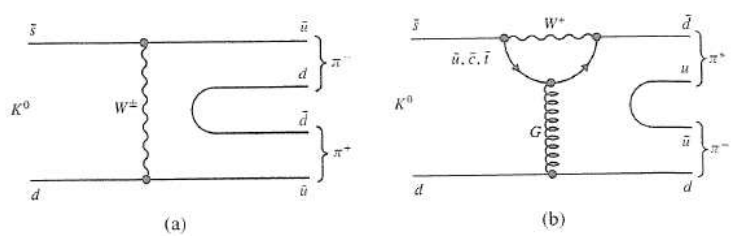
\includegraphics[scale=0.3]{figs/Perkins_Interference_Kaons.png}
\end{center}
\caption{\textit{Two possible decay modes for $K^{0} \rightarrow \pi^+ \pi^-$. (a) Tree diagram for decay by exchanging W boson (b) Penguin diagram for decay via quark states \cite{HEPP_intro_Perkins}}}
\label{HEPP_intro_Perkins}
\end{figure}

\noindent However it is found that the direct CPV contribution is much smaller in this case. The indirect CPV almost completely dominates as can be seen from the similarity of the experimental values for $|\eta_{+-}|$ and $|\eta_{00}|$ \cite{PDGKaons}:

\begin{align*}
|\eta_{00}| = 0.002220 \pm 0.000011 &  & |\eta_{+-}| = 0.002232 \pm 0.000011 
\end{align*}  

\noindent If these values were significantly different it would suggest the amount of direct CPV would be comparable to the amount of indirect CPV, this of course is not the case. An experimentally determined value which illustrates this is the real part of the ratio of $\epsilon'$ to $epsilon$ \cite{PDGKaons}:

\begin{equation*}
\mathbb{R} \big(\frac{\epsilon'}{\epsilon} \big)  = \big(1 - \big|\frac{\eta_{00}}{\eta{+-}}\big|\big) / 3 = 0.00166 \pm 0.00023
\end{equation*}

\noindent We can also determine $|\epsilon|$ using:

\begin{equation*} 
|\epsilon| = (2 |\eta_{+-}| + |\eta_{00}|)/3 = 0.002228 \pm 0.000011
\end{equation*} 


\noindent If we ignore the direct CPV contributions we can write Eqn.(\ref{KaonLincomb11}) and (\ref{KaonLincomb12}) in terms of $\epsilon$:

\begin{align}
\label{KaonLincomb21}
\ket{K^{0}_{L}} = \frac{1}{(1+|\epsilon|^2)^{1/2}} \big[ \epsilon \ket{K^{0}_{1}} + \ket{K^{0}_{2}} \\
\label{KaonLincomb22}
\ket{K^{0}_{S}} = \frac{1}{(1+|\epsilon|^2)^{1/2}} \big[ \ket{K^{0}_{1}} - \epsilon \ket{K^{0}_{2}}
\end{align}

\noindent Thus we have a linear combination which shows the non-zero amplitude for a state with definite $CP$ to osciallate and decay into final states with the opposite CP.

\subsection{Semi-leptonic decays}

Decays of neutral Kaons to products containing leptons can be used to verify Eqn.(\ref{KaonLincomb21}) and (\ref{KaonLincomb22}) as well as finding the asymmetry in the Kaon oscillation $K^{0} \leftrightarrow \bar{K}^{0}$. First we must discuss the selection rules that play an important role in these decays.

The $\Delta S = \Delta Q$ selection rule is an empirical rule backed up by some theoretical approximations. This rules states that in decays involving strangeness(S) and leptons, the change in the charge(Q) of the hadrons must be the same as the change in strangeness which must have a value of $\pm 1$. We first look at semi-leptonic decays of the charged $\Sigma$ baryon. Two semi-leptonic decays of this baryon are:

\begin{align}
\label{Sigma1}
\Sigma^{-} (dds) \rightarrow n(udd) + e^{-} + \bar{\nu}_{e} \\
\label{Sigma2}
\Sigma^{+} (uus) \rightarrow n(udd) + e^{+} + \nu_{e}
\end{align}  

\noindent The feynmann diagram for decay (\ref{Sigma1}) can be drawn as in Fig.(pg232 M+S[use jaxo or others know how feynmann latex??]), while decay (\ref{Sigma2}) requires a diagram such as Fig.(Two W decay). It is clear that the diagram for $\Sigma^{-}$ is quite likely as it contains the Cabbibo favoured quark coupling $V_{ud}$ while the digram for $\Sigma^{+}$ is very unlikely. In fact, the decay (\ref{Sigma2}) must always contain at least two W bosons, as there are two quark flavour changes in the decay. For this reason it is highly suppressed and has a braching ratio of $< (5\e{-6})$, which is consitent with it not existing in nature \cite{PDGKaons}. In comparrison the decay (\ref{Sigma1}) has a branching ratio of $(1.017 \pm 0.034) \e{-3}$. As there is no selection rule forbidding this decay, the $\Delta S = \Delta Q$ rule was introduced to identify these types of decays. 


